\textit{Alvarenga p646 - Ejercicio 3}\\Un rayo luminoso RO incide sobre un espejo plano colocado en la posición EO, como se muestra en la figura de este problema. Siendo ON la normal a este espejo.
\begin{enumerate}
    \item Trace cuidadosamente en la figura el rayo reflejado OR' (use un transportador para medir los ángulos).
    \item El espejo se gira un ángulo $\alpha = 15^\circ$, colocándose en la nueva posición E'O (véase figura). Trace la normal ON' para esta nueva posición del espejo.
    \item Considerando el mismo rayo incidente, trace el rayo reflejado, OR'', para la posición E'O del espejo.
    \item Mida con el transportador el ángulo $\beta$ que giró el rayo reflejado al pasar de la posición OR' a OR''.
    \item Se puede demostrar que $\beta = 2 \alpha$, es decir cuando un espejo plano gira cierto ángulo, el rayo reflejado gira un ángulo dos veces mayor. ¿Sus medidas concuerdan con este resultado? 
\end{enumerate}
\begin{figure}[h!]
\centering
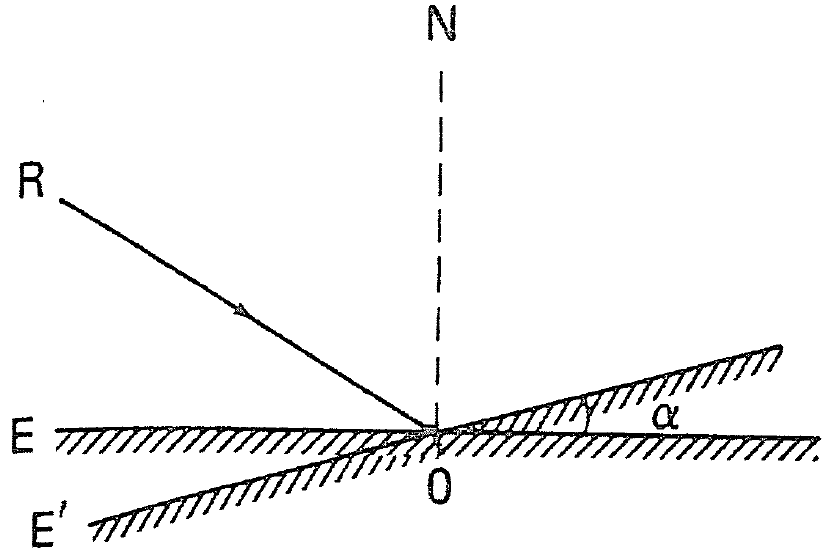
\includegraphics[width=0.37\linewidth]{problema3_alvarenga646.png}
 \caption{Problema 7}
\end{figure}